\begin{figure}

  \begin{center}
  % %%%%%%%%%%%%%%%%%%%%%%%%%%%%%%%%%%%%%%%%%%%%%%%%%%%%%%%%
  Hierarchical Clustering \\
  \begin{minipage}{0.20\textwidth}
    % \begin{center}
      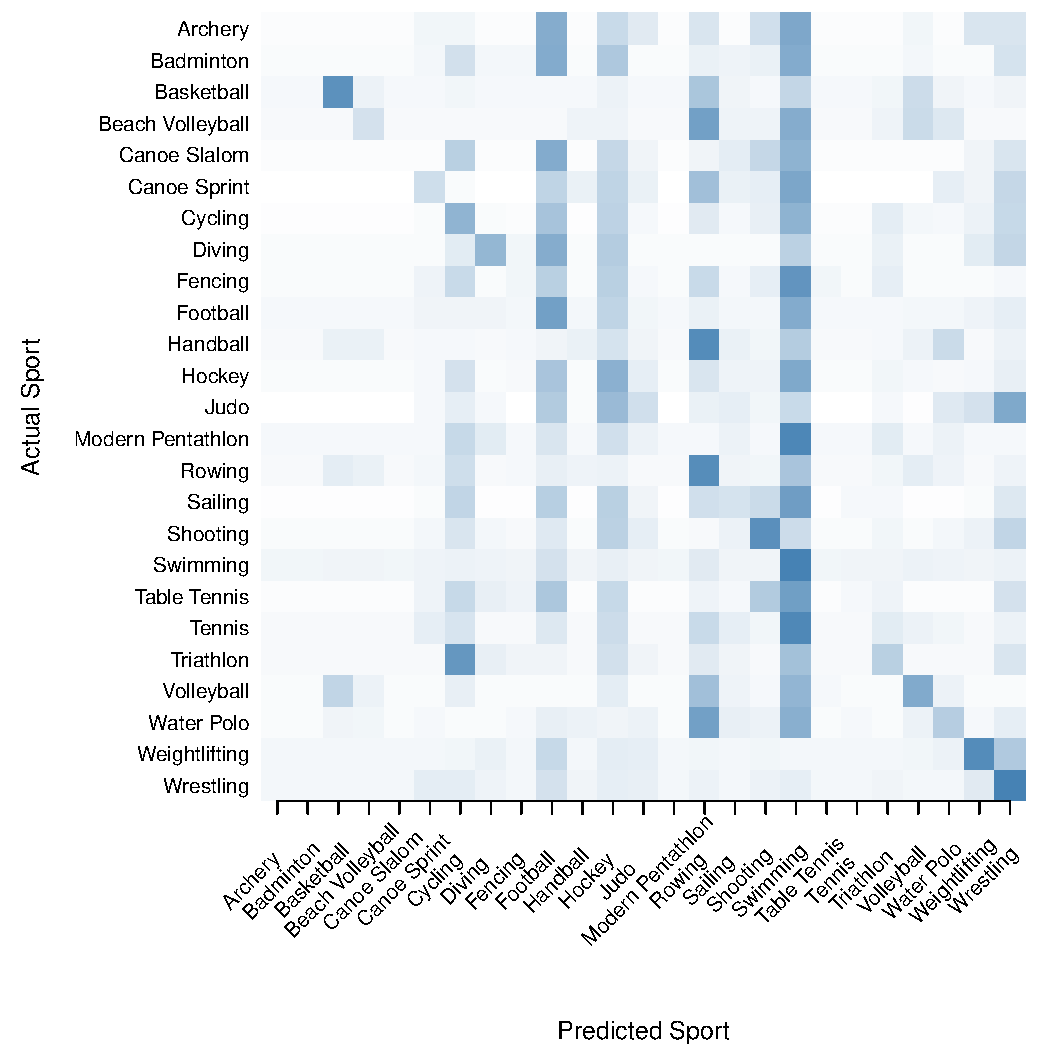
\includegraphics[scale=0.20]{../graphics/sportMclust-trn.pdf}
    % \end{center}
  \end{minipage}
  \hspace{0.05\textwidth}
  \begin{minipage}{0.20\textwidth}
    % \begin{center}
      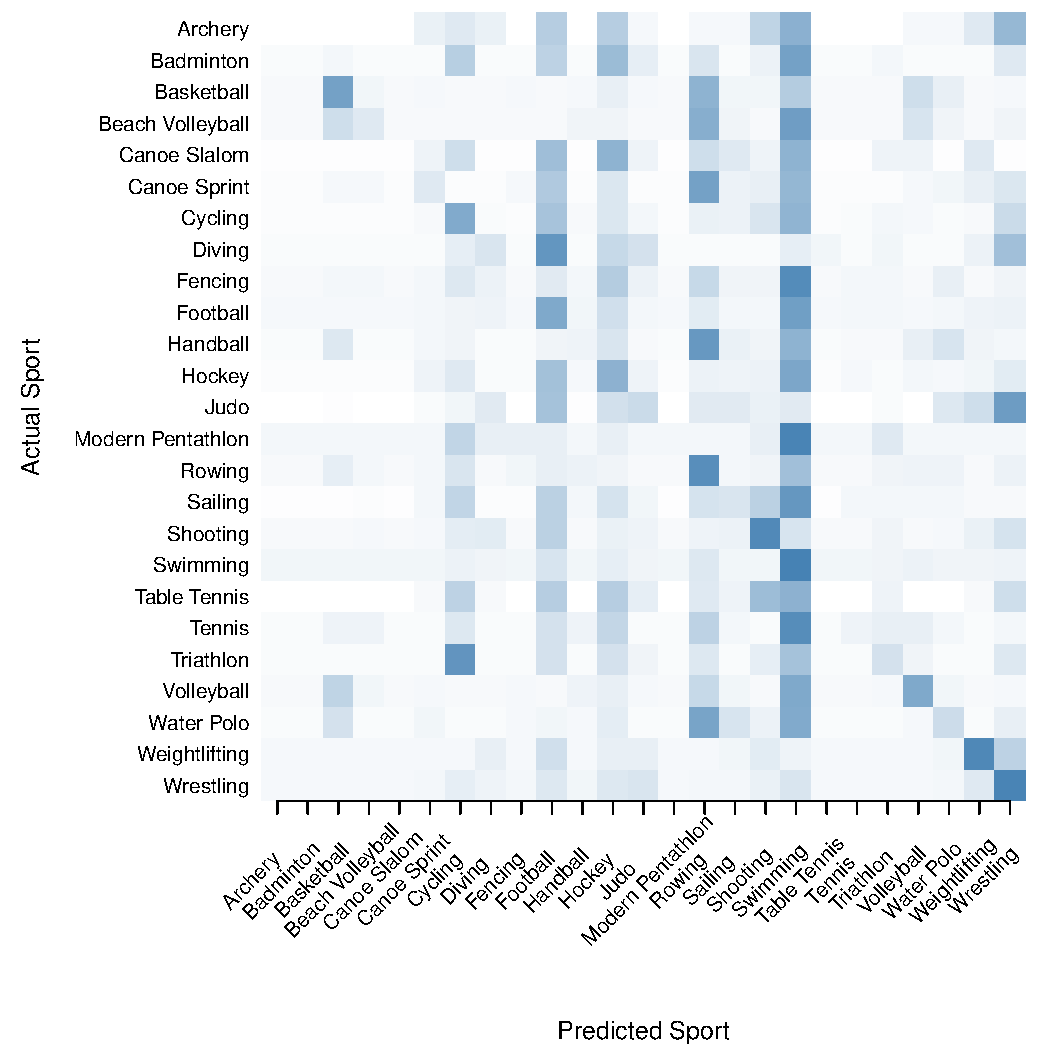
\includegraphics[scale=0.20]{../graphics/sportMclust-tst.pdf}
    % \end{center}
  \end{minipage}
  \hspace{0.05\textwidth}
  \begin{minipage}{0.20\textwidth}
    \hspace{1.0in}
  \end{minipage}
  \hspace{0.05\textwidth}
  \begin{minipage}{0.20\textwidth}
    \begin{center}
      \hspace{0.11in} Legend\\
      \hspace{-0.1in} 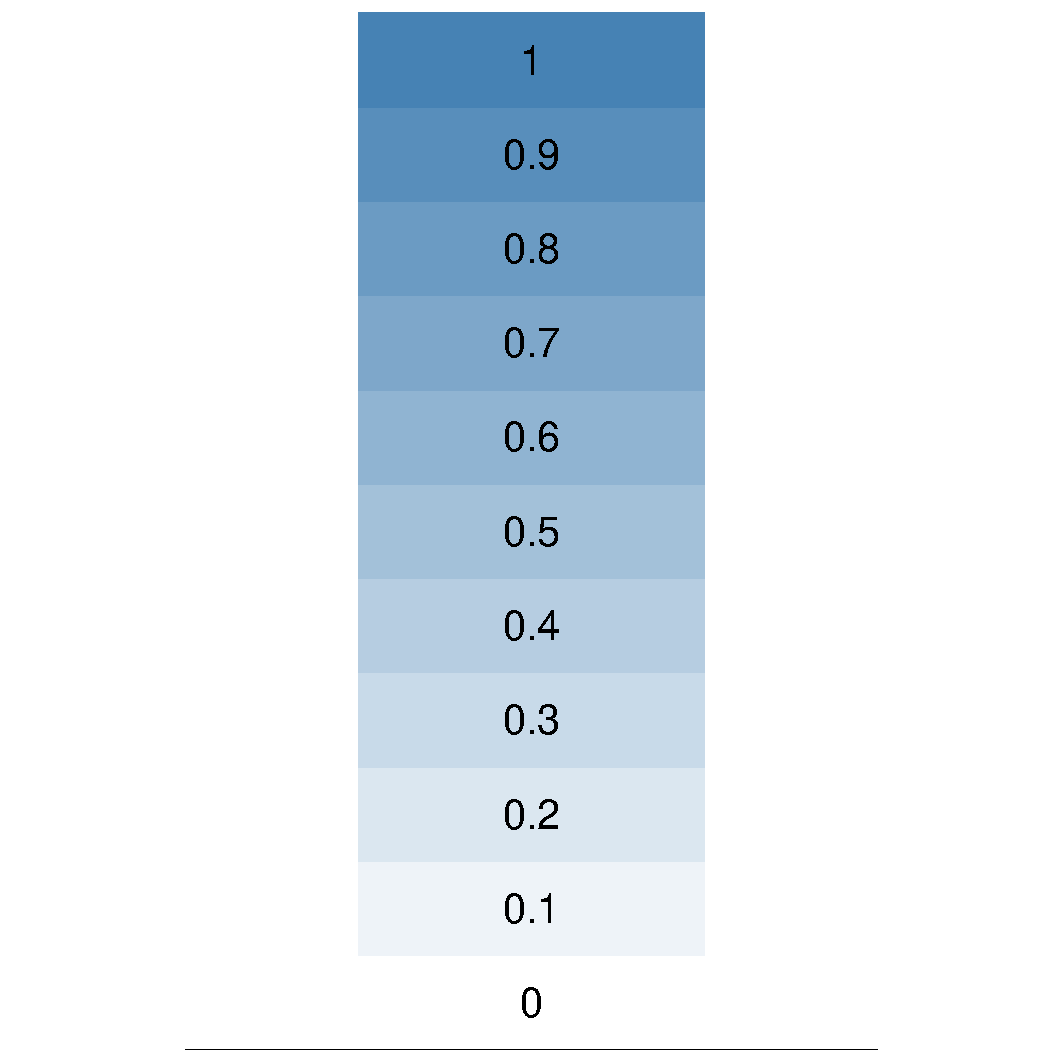
\includegraphics[scale=0.20]{../graphics/scale.pdf}  
    \end{center}
  \end{minipage}




  %%%%%%%%%%%%%%%%%%%%%%%%%%%%%%%%%%%%%%%%%%%%%%%%%%%%%%%%%
    Conditional Inference Tree \\

  \begin{minipage}{0.20\textwidth}
    \begin{center}
      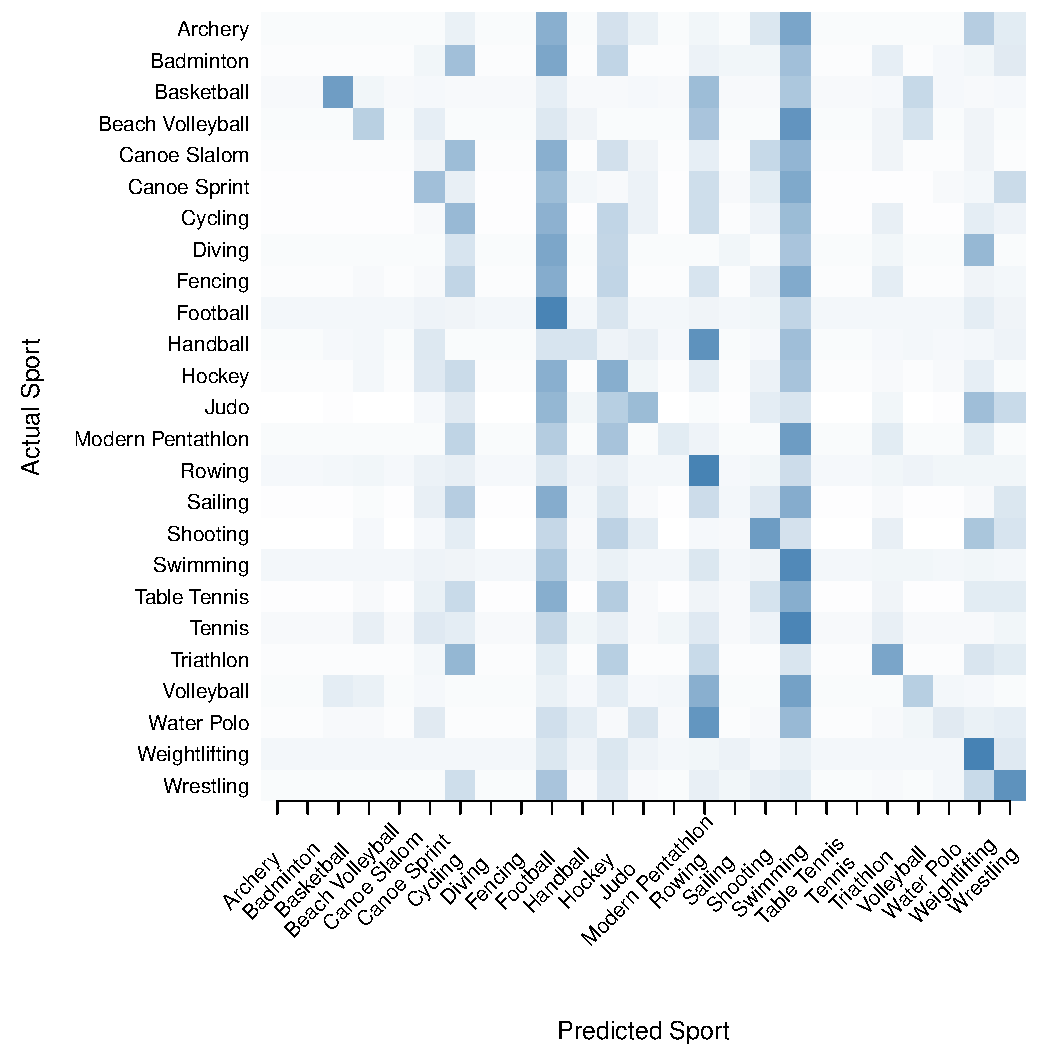
\includegraphics[scale=0.20]{../graphics/sportCIT-trn.pdf}
    \end{center}
  \end{minipage}
  \hspace{0.05\textwidth}
  \begin{minipage}{0.20\textwidth}
    \begin{center}
      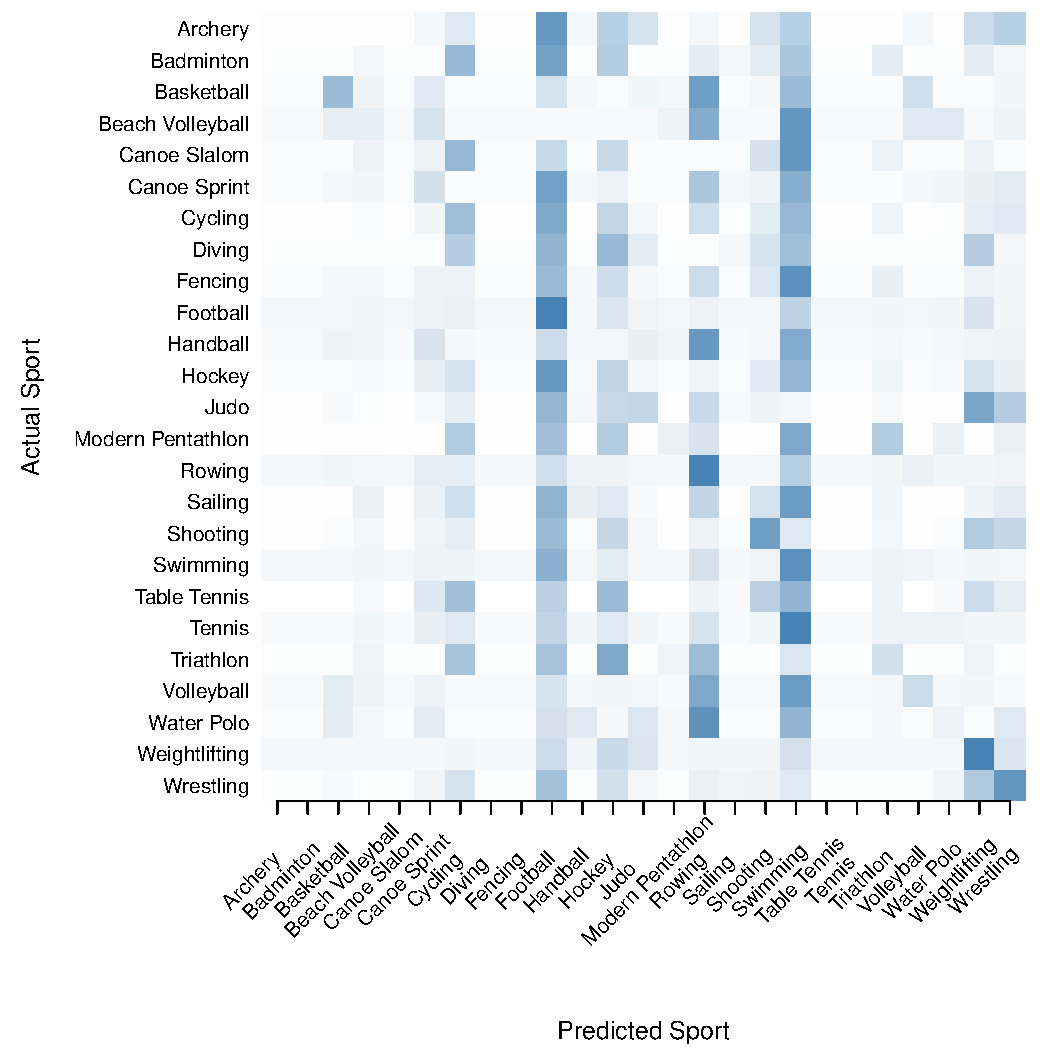
\includegraphics[scale=0.20]{../graphics/sportCIT-tst.pdf}
    \end{center}
  \end{minipage}
  \hspace{0.05\textwidth}
    \begin{minipage}{0.20\textwidth}
    \begin{center}
      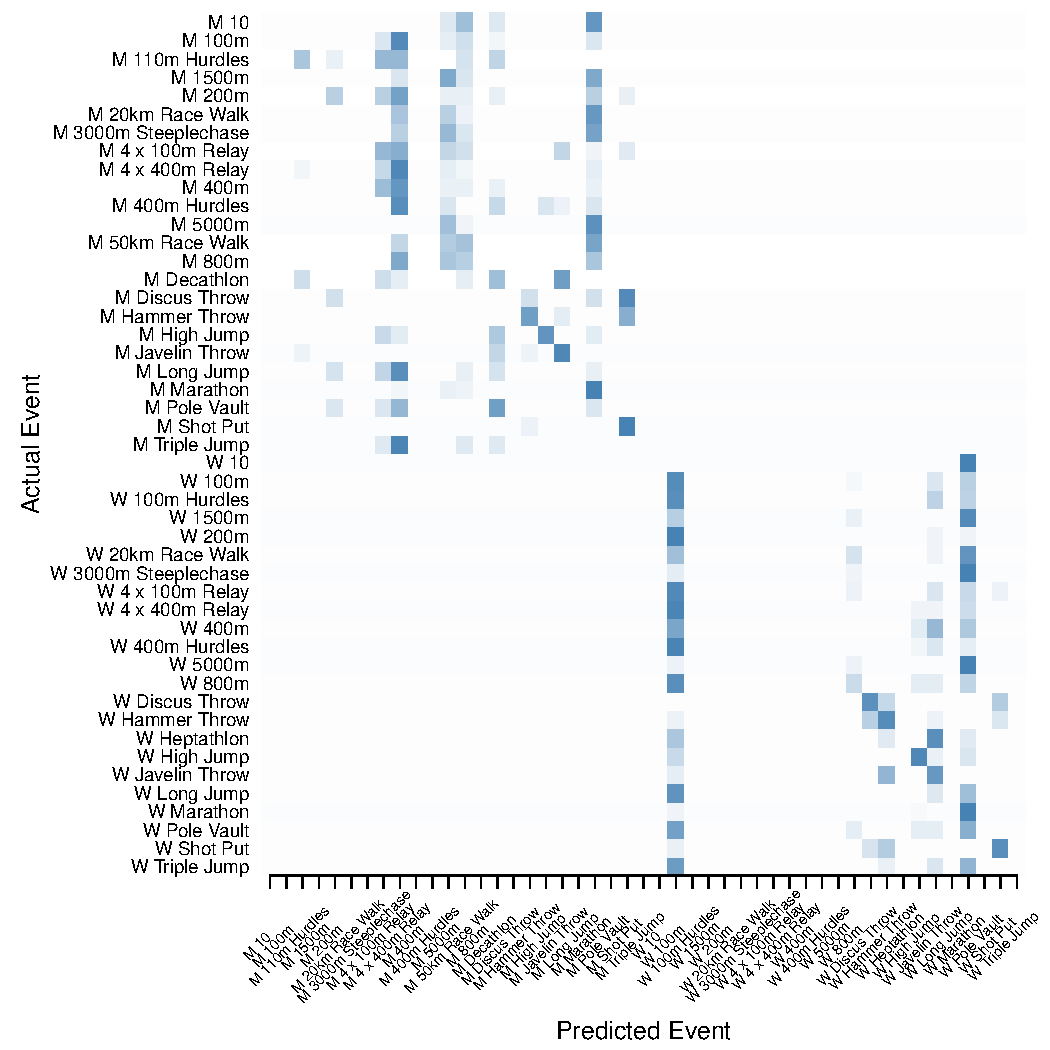
\includegraphics[scale=0.20]{../graphics/athletesCIT-trn.pdf}
    \end{center}
  \end{minipage}
  \hspace{0.05\textwidth}
  \begin{minipage}{0.20\textwidth}
    \begin{center}
      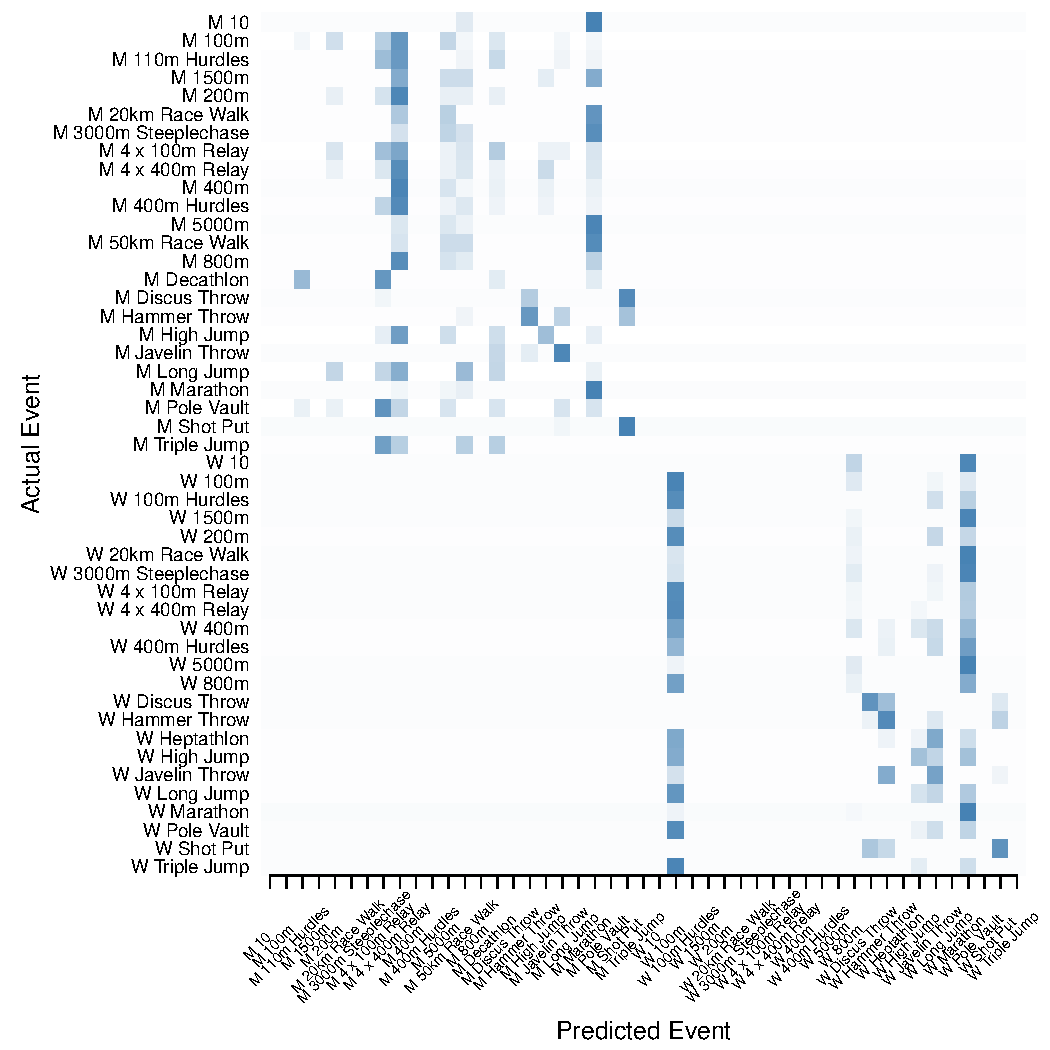
\includegraphics[scale=0.20]{../graphics/athletesCIT-tst.pdf}
    \end{center}
  \end{minipage}



  %%%%%%%%%%%%%%%%%%%%%%%%%%%%%%%%%%%%%%%%%%%%%%%%%%%%%%%%%
    Evolutionary Tree \\

  \begin{minipage}{0.20\textwidth}
    \begin{center}
      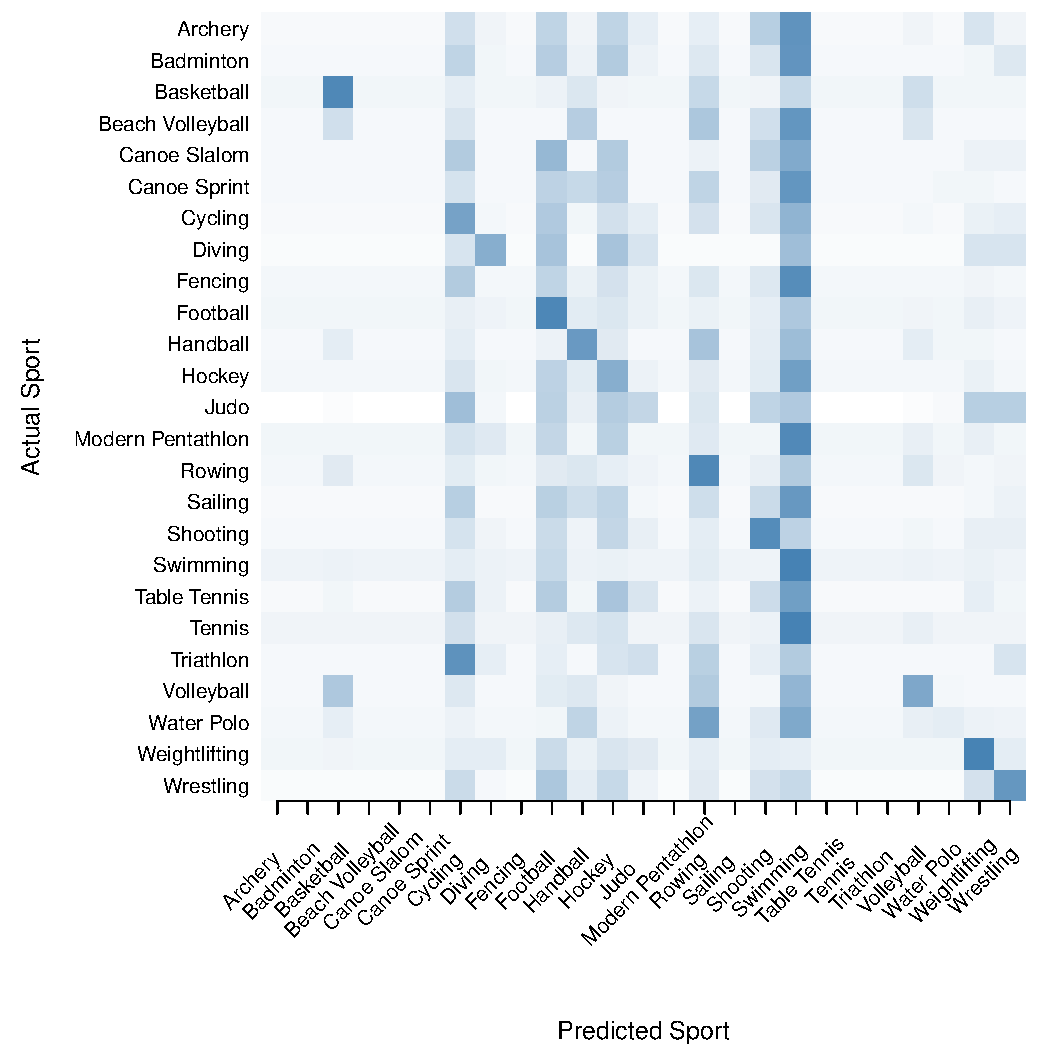
\includegraphics[scale=0.20]{../graphics/sportEV-trn.pdf}
    \end{center}
  \end{minipage}
  \hspace{0.05\textwidth}
  \begin{minipage}{0.20\textwidth}
    \begin{center}
      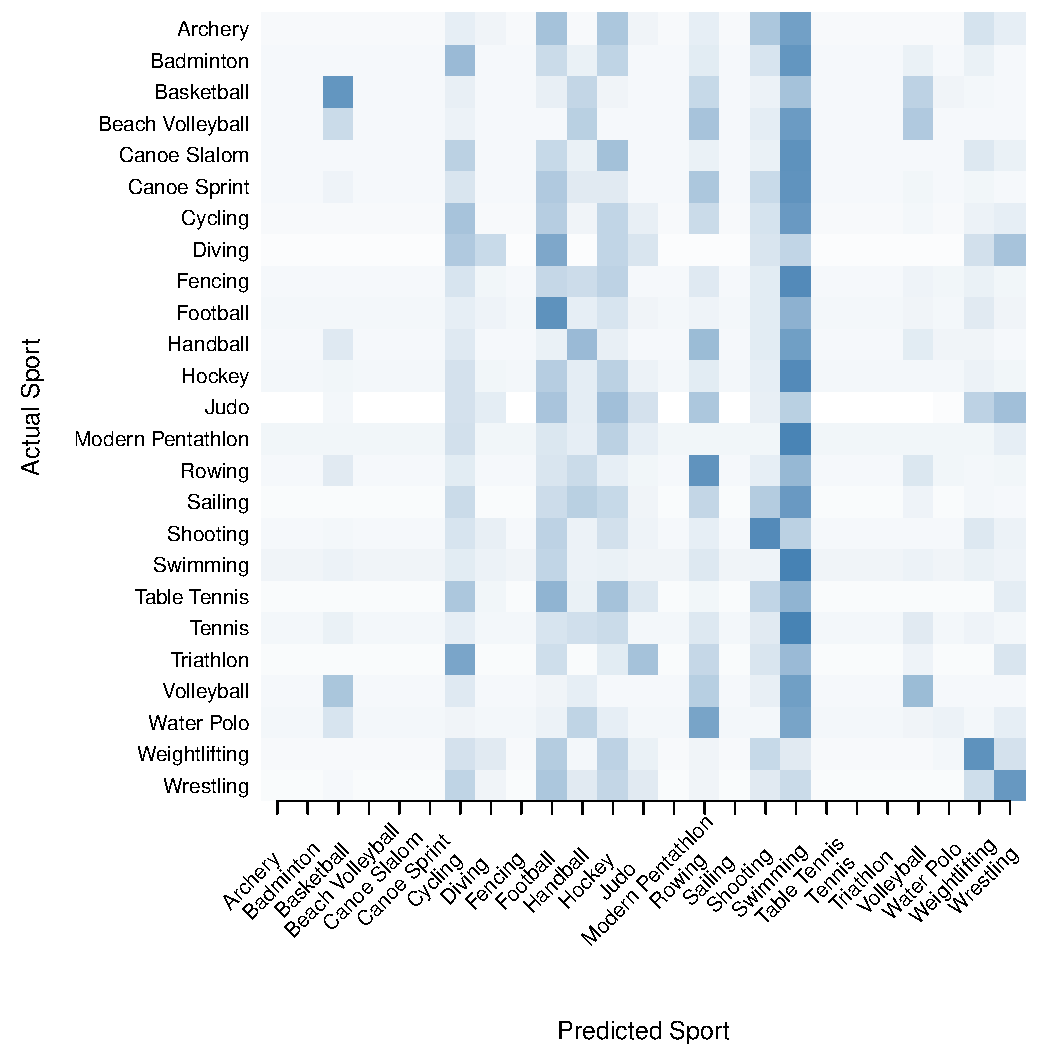
\includegraphics[scale=0.20]{../graphics/sportEV-tst.pdf}
    \end{center}
  \end{minipage}
  \hspace{0.05\textwidth}
    \begin{minipage}{0.20\textwidth}
    \begin{center}
      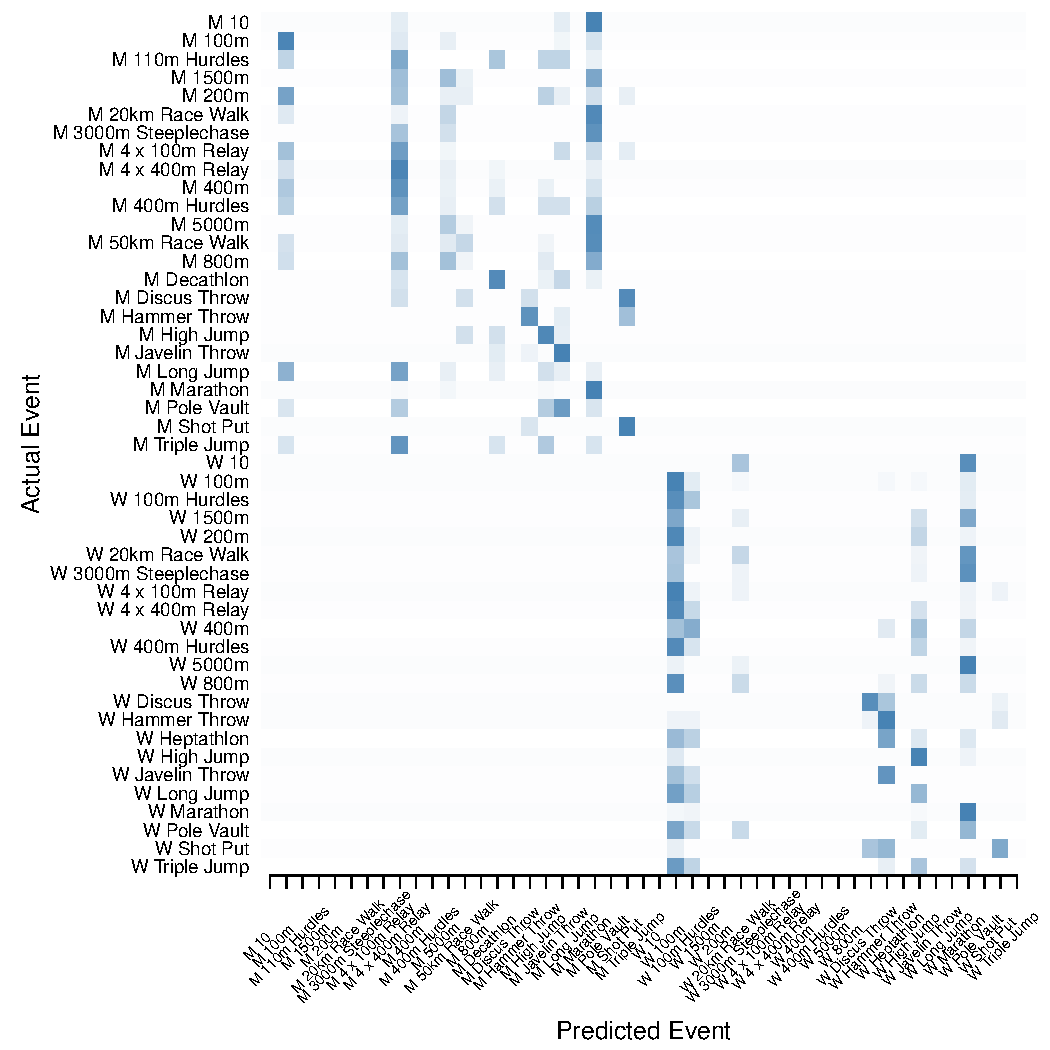
\includegraphics[scale=0.20]{../graphics/athletesEV-trn.pdf}
    \end{center}
  \end{minipage}
  \hspace{0.05\textwidth}
  \begin{minipage}{0.20\textwidth}
    \begin{center}
      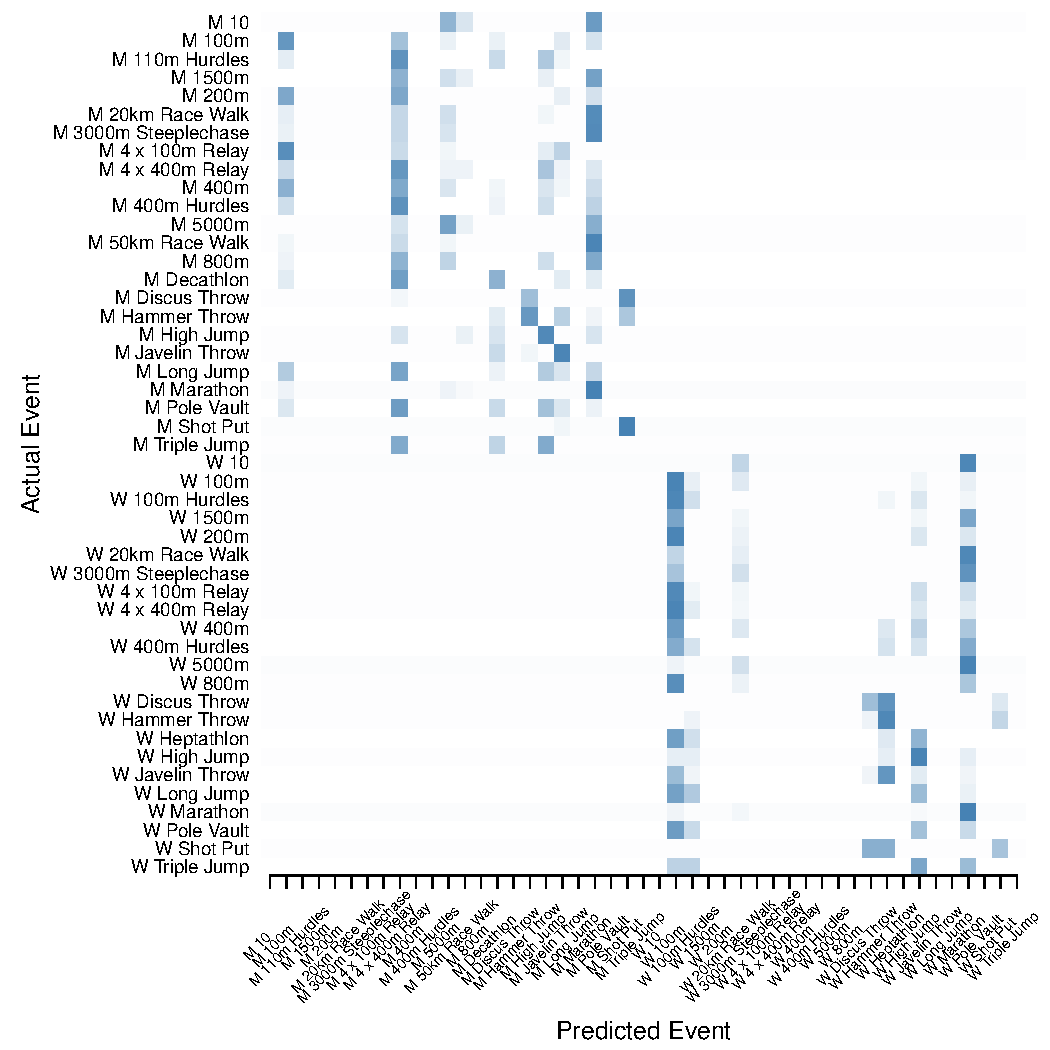
\includegraphics[scale=0.20]{../graphics/athletesEV-tst.pdf}
    \end{center}
  \end{minipage}


  %%%%%%%%%%%%%%%%%%%%%%%%%%%%%%%%%%%%%%%%%%%%%%%%%%%%%%%%%
    Random Forest \\
  \begin{minipage}{0.20\textwidth}
    \begin{center}
      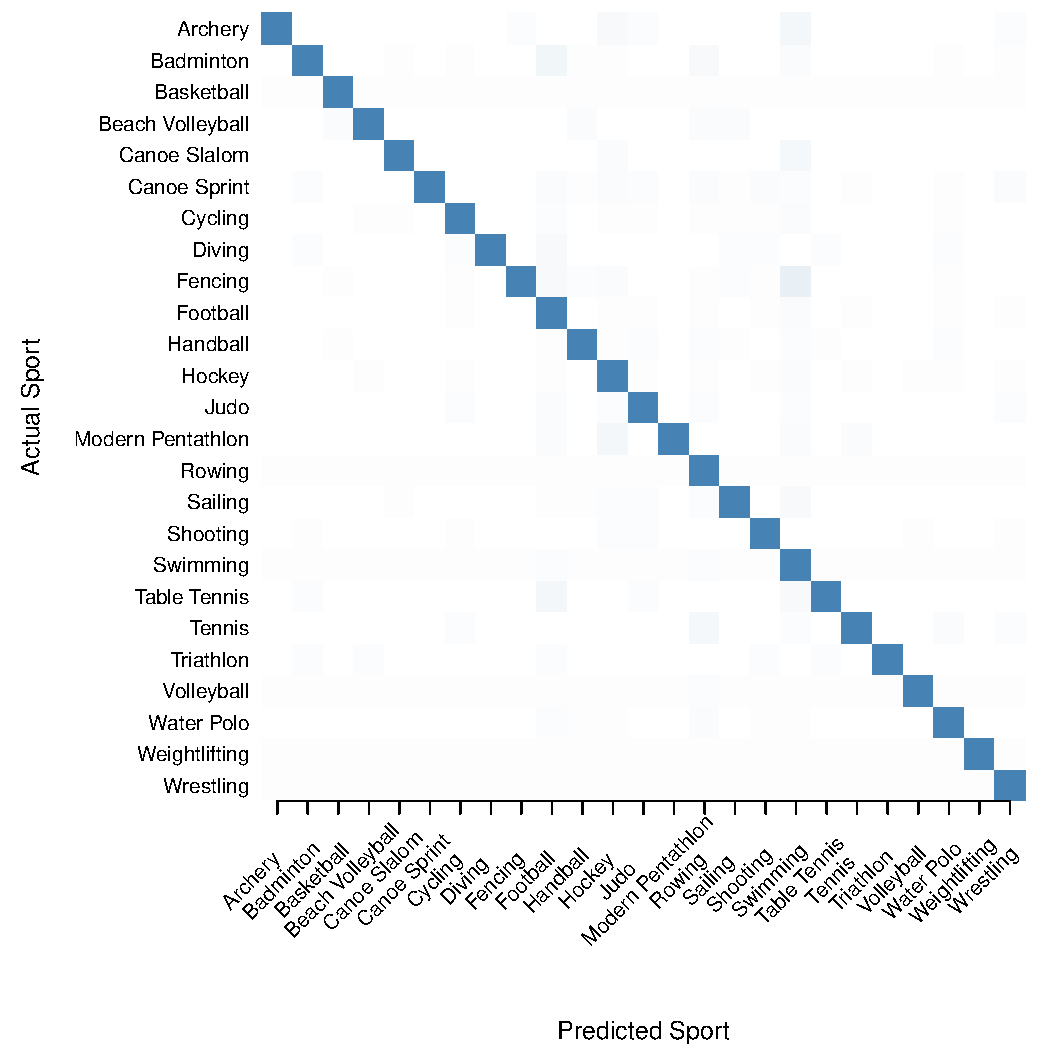
\includegraphics[scale=0.20]{../graphics/sportRF-trn.pdf}
    \end{center}
  \end{minipage}
  \hspace{0.05\textwidth}
  \begin{minipage}{0.20\textwidth}
    \begin{center}
      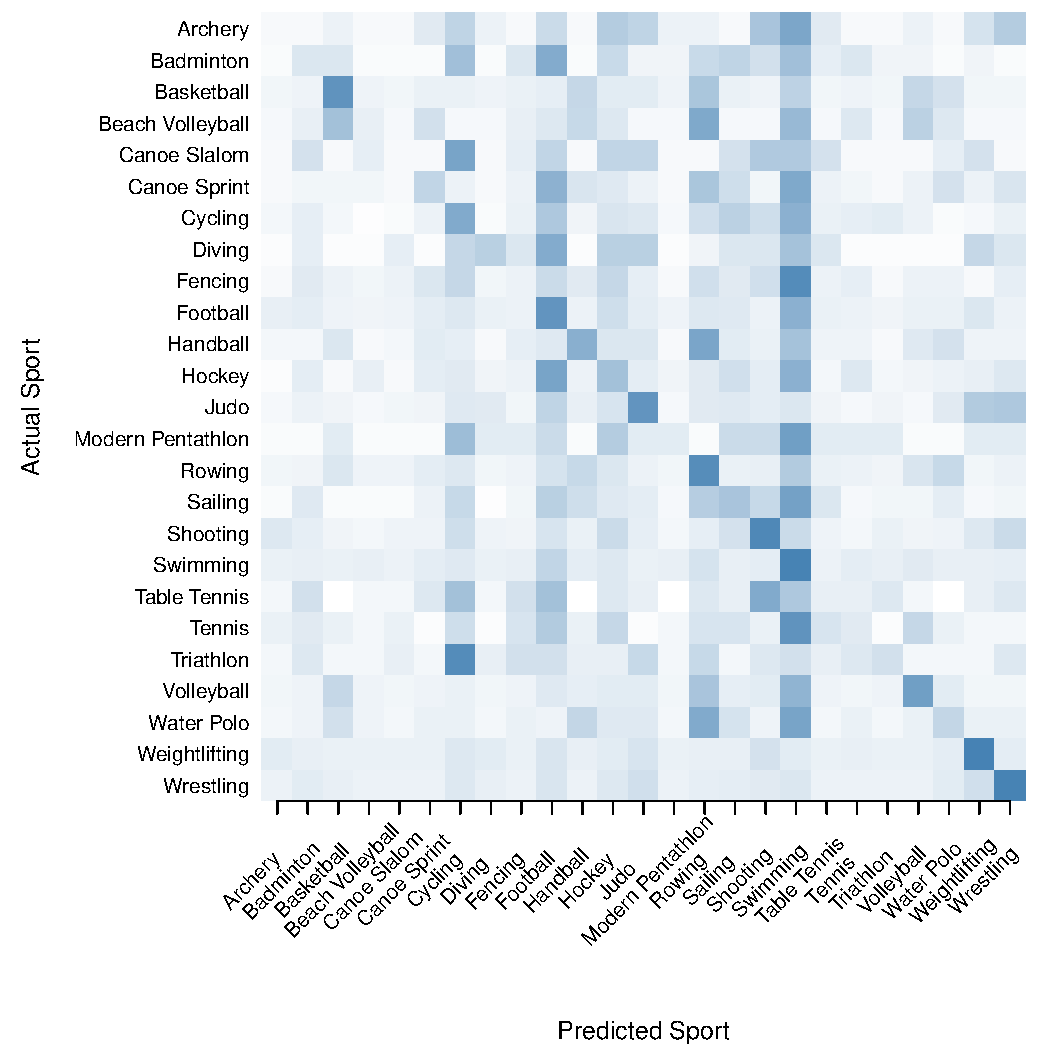
\includegraphics[scale=0.20]{../graphics/sportRF-tst.pdf}
    \end{center}
  \end{minipage}
    \hspace{0.05\textwidth}
    \begin{minipage}{0.20\textwidth}
    \begin{center}
      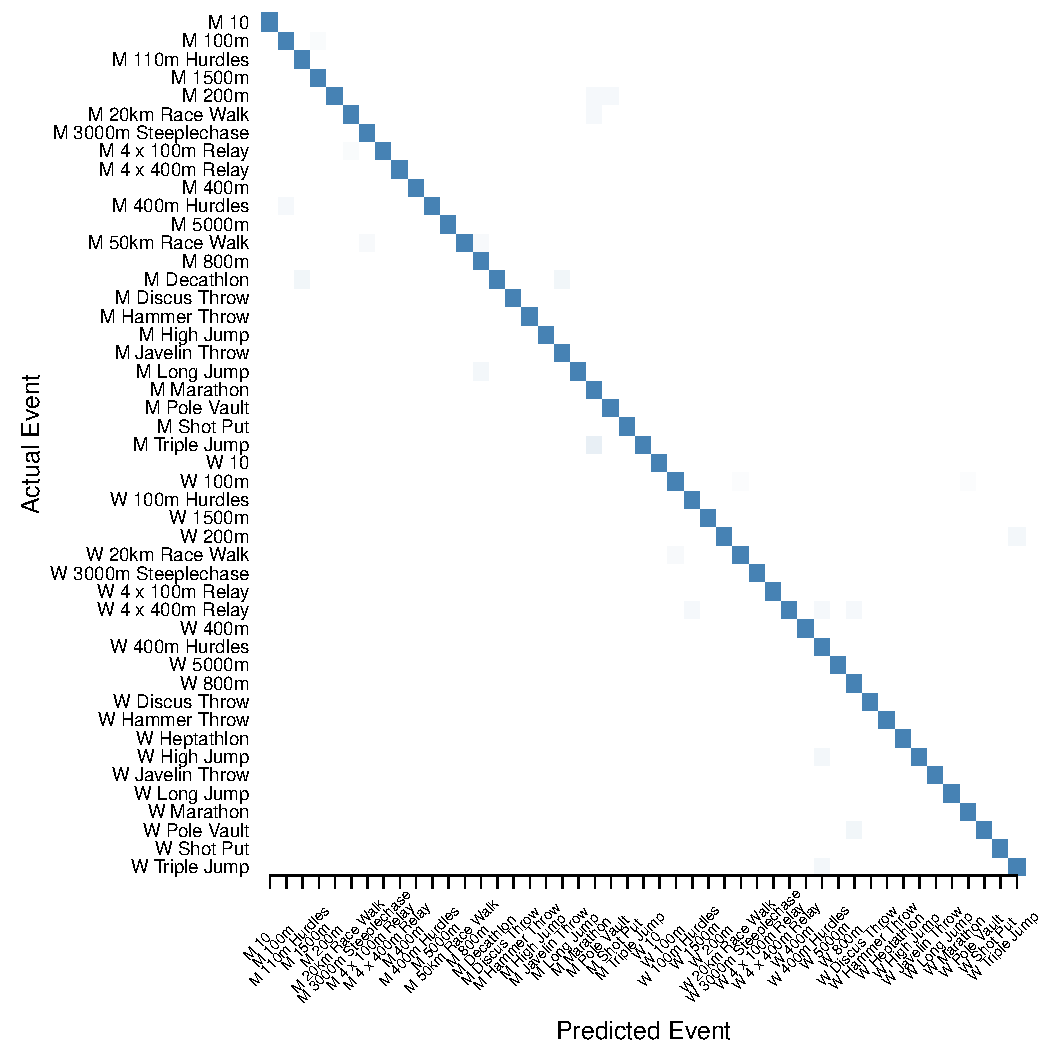
\includegraphics[scale=0.20]{../graphics/athletesRF-trn.pdf}
    \end{center}
  \end{minipage}
  \hspace{0.05\textwidth}
  \begin{minipage}{0.20\textwidth}
    \begin{center}
      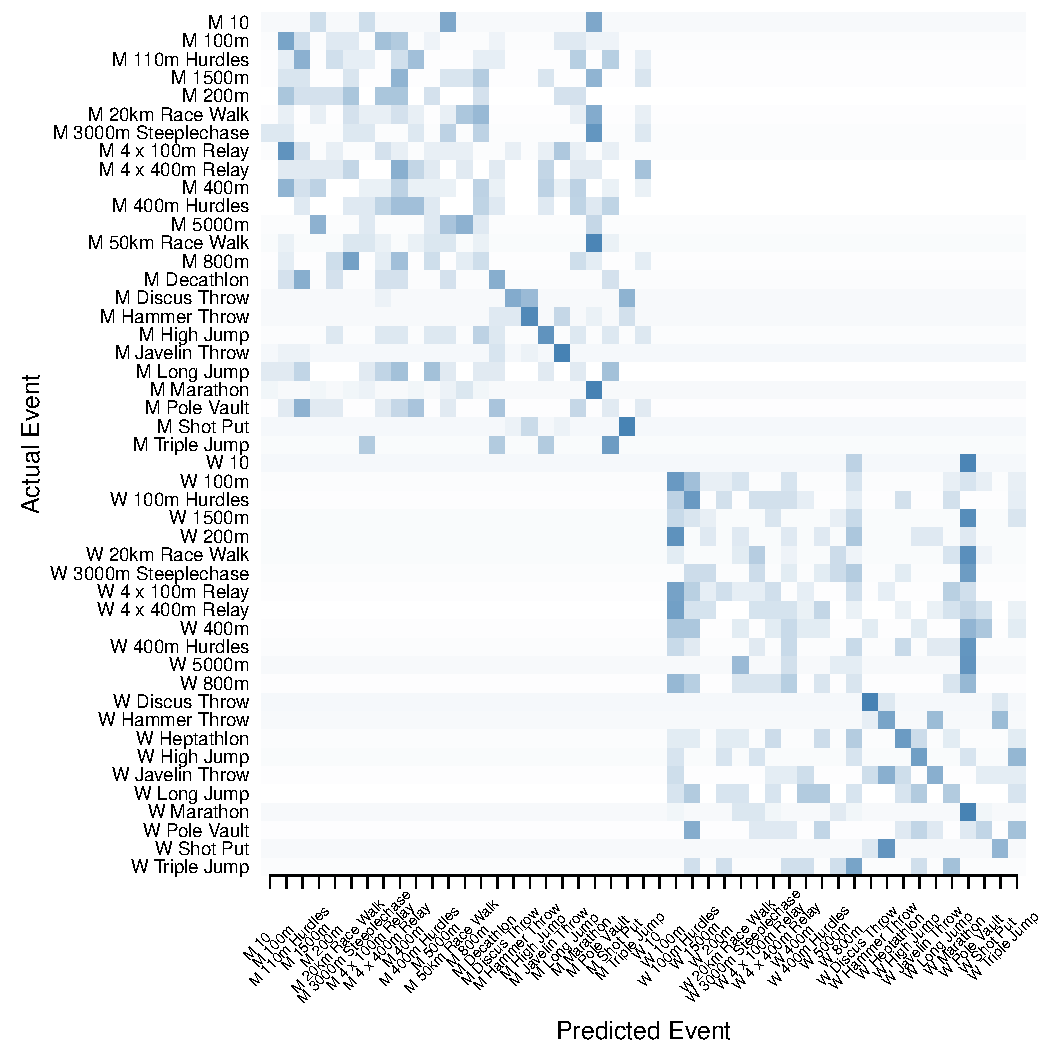
\includegraphics[scale=0.20]{../graphics/athletesRF-tst.pdf}
    \end{center}
  \end{minipage}



  %%%%%%%%%%%%%%%%%%%%%%%%%%%%%%%%%%%%%%%%%%%%%%%%%%%%%%%%%
    Neural Network \\
  \begin{minipage}{0.20\textwidth}
    \begin{center}
      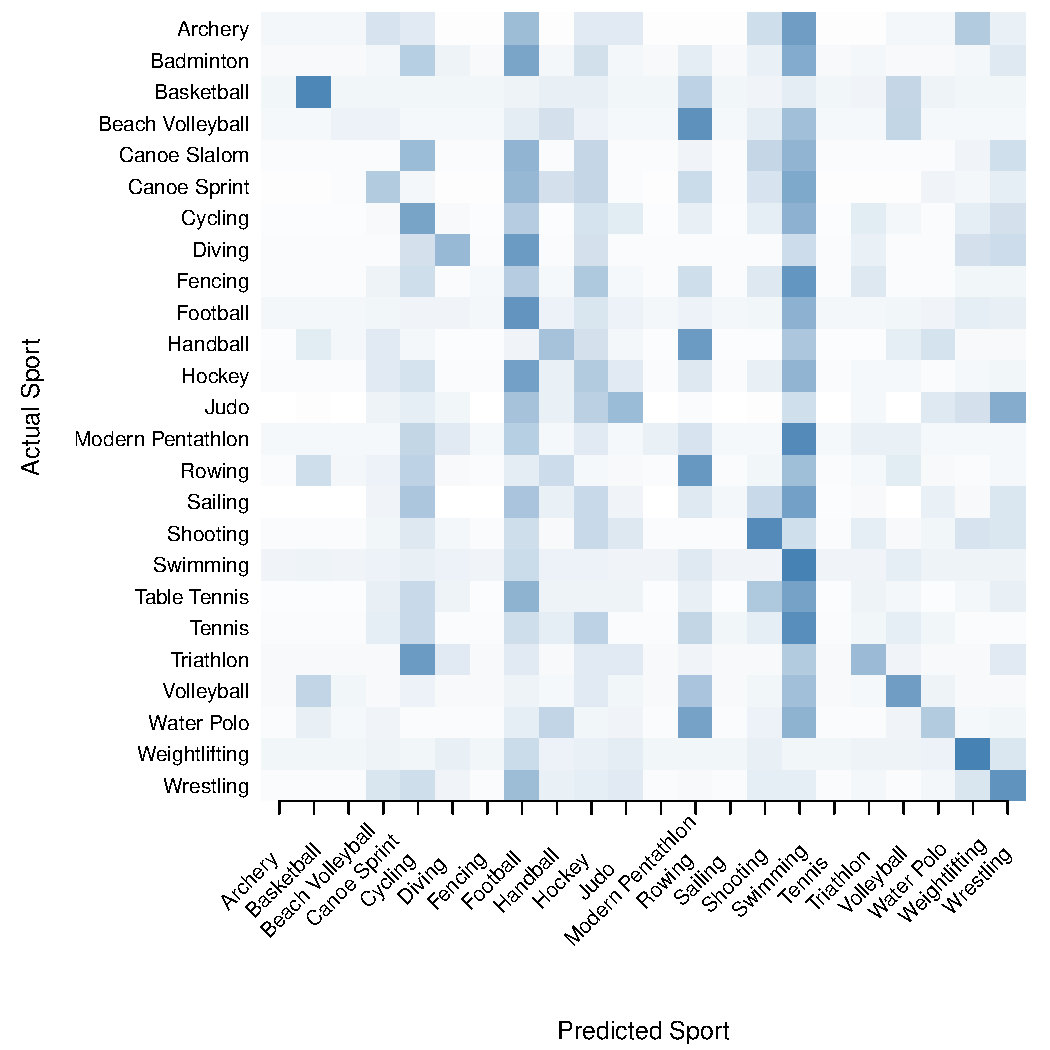
\includegraphics[scale=0.20]{../graphics/sportANN-trn.pdf}
    \end{center}
  \end{minipage}
  \hspace{0.05\textwidth}
  \begin{minipage}{0.20\textwidth}
    \begin{center}
      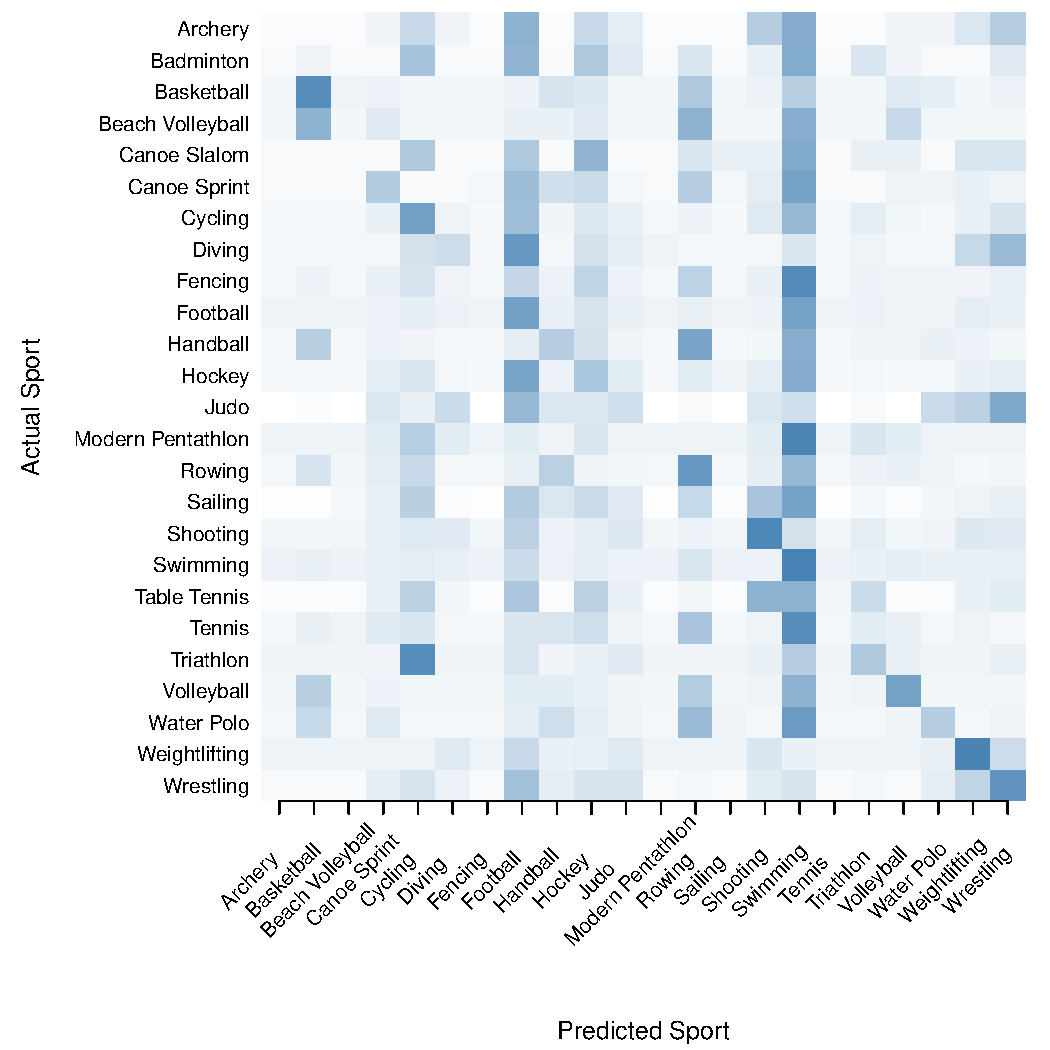
\includegraphics[scale=0.20]{../graphics/sportANN-tst.pdf}
    \end{center}
  \end{minipage}
    \hspace{0.05\textwidth}
    \begin{minipage}{0.20\textwidth}
    \begin{center}
      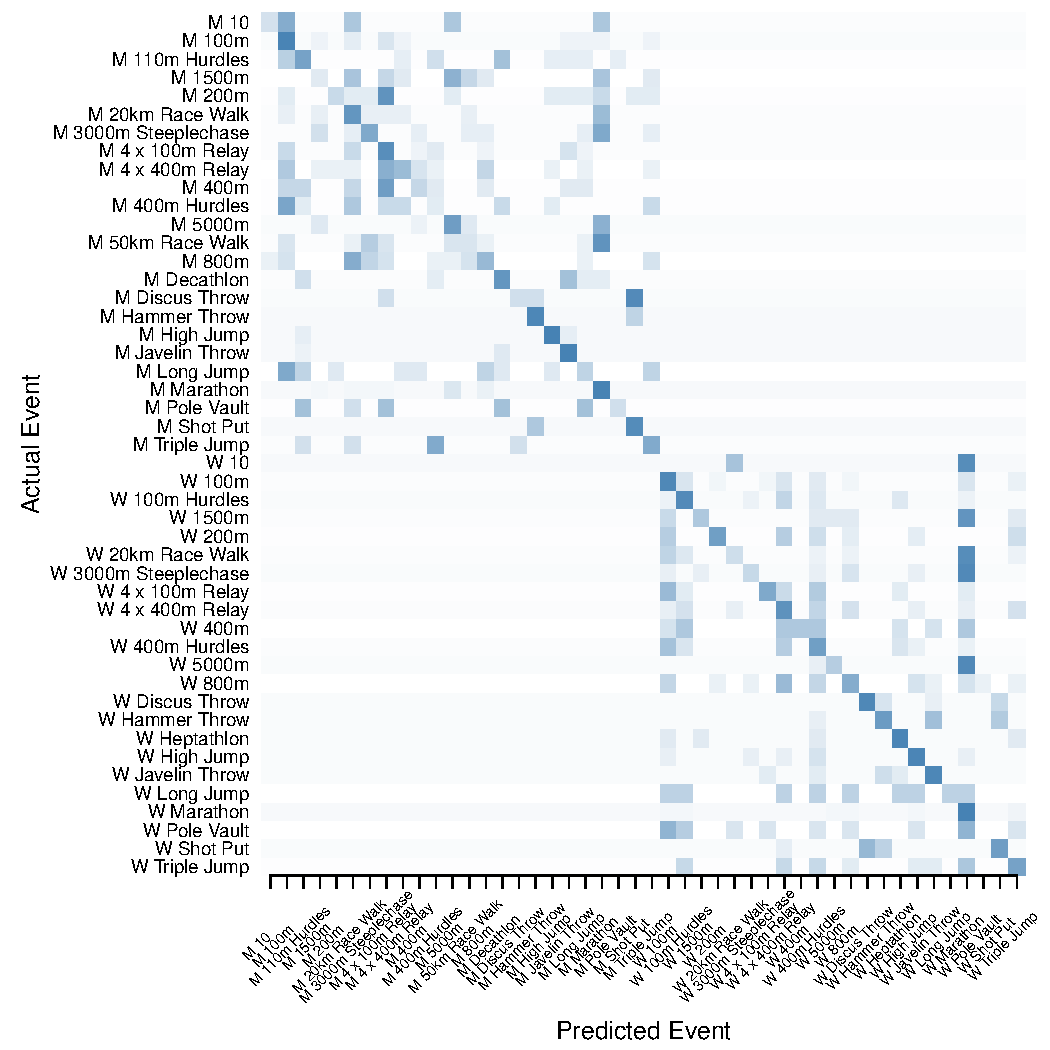
\includegraphics[scale=0.20]{../graphics/athletesANN-trn.pdf}
    \end{center}
  \end{minipage}
  \hspace{0.05\textwidth}
  \begin{minipage}{0.20\textwidth}
    \begin{center}
      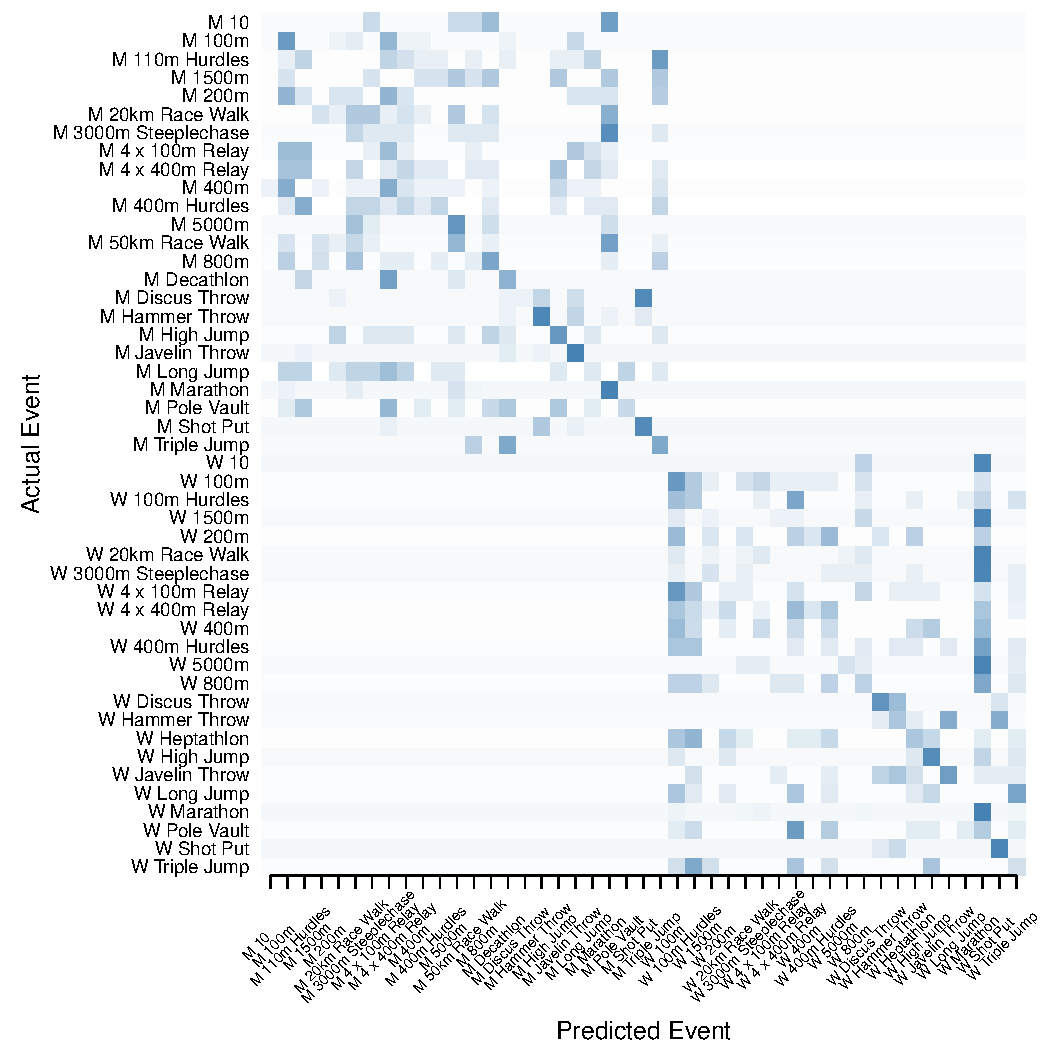
\includegraphics[scale=0.20]{../graphics/athletesANN-tst.pdf}
    \end{center}
  \end{minipage}

  \end{center}

\caption{Classification matrices by method for sports (left two columns) and events (right two columns). The first and third columns present results using the training sets for the respective classification tasks, and the second and fourth columns are results using the corresponding test sets. Participants' actual sports/events are labeled on the rows of each image, and the predicted sports/events are labeled on the columns. The cells represent row-normalized frequencies. Darker shades on the diagonal indicate accurate classification.}
\label{matrices}
\end{figure}